%!TEX root = ../booklet.tex
% ^ leave for LaTeXTools build functionality

\begin{puzzle}
  \rightImg{2in}{balancingAct/scaleIllustration.pdf}
  The labels on the following scales can be rearranged to spell out a clue
  to the location of an EXTRA Puzzle. These rules will tell you how to
  rearrange the letters:

  \begin{itemize}
  \item These are balance scales, so the total weights on each side of a scale
        are exactly the same.
  \item The kettlebells $A$, $B$, $C$, $D$ are the same for each picture,
        with $A$ being the lightest to $D$ being the heaviest.
  \item The $?$ kettlebell is always a unique weight between $1$ and $40$ from
        picture to picture.
  \end{itemize}

  \vfill

  \begin{center}
    \letterBox{1}
    \letterBox{2}
    \letterBox{3}
    \hspace{2em}
    \letterBox{4}
    \letterBox{5}
    \letterBox{6}
    \hspace{2em}
    \letterBox{7}
    \letterBox{8}
    \letterBox{9}
    \letterBox{10}
    \letterBox{11}

    \letterBox{12}
    \letterBox{13}
    \letterBox{14}
    \letterBox{15}
    \letterBox{16}
    \letterBox{17}
    \letterBox{18}
    \hspace{2em}
    \letterBox{19}
    \letterBox{20}
    \letterBox{21}

    \letterBox{22}
    \letterBox{23}
    \letterBox{24}
    \letterBox{25}
    \hspace{2em}
    \letterBox{26}
    \letterBox{27}
    \letterBox{28}

    \letterBox{29}
    \letterBox{30}
    \letterBox{31}
    \letterBox{32}
    \letterBox{33}
    \letterBox{34}
    \letterBox{35}
    \letterBox{36}
    \hspace{2em}
    \letterBox{37}
    \letterBox{38}
    \letterBox{39}
    \letterBox{40}
  \end{center}

  Report the correctly decoded message above to Game HQ for \(100\) points!

  \vfill

  \newpage

  \begin{center}
    \begin{tabular}{c}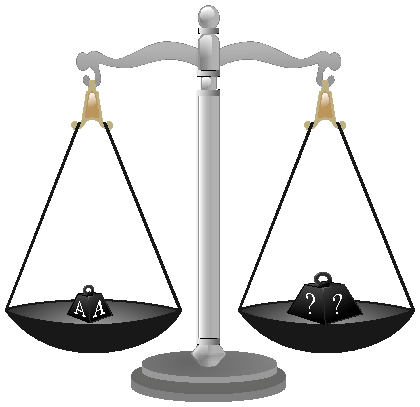
\includegraphics[width=0.2\linewidth]{balancingAct/balanceScale01.pdf}\\Y\end{tabular}
    \begin{tabular}{c}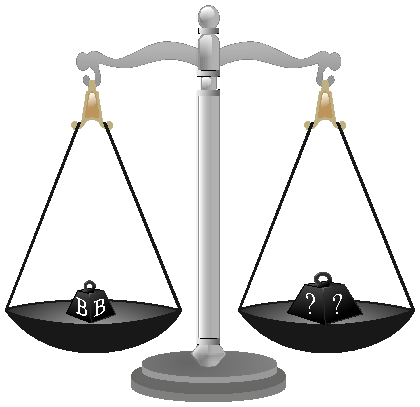
\includegraphics[width=0.2\linewidth]{balancingAct/balanceScale03.pdf}\\U\end{tabular}
    \begin{tabular}{c}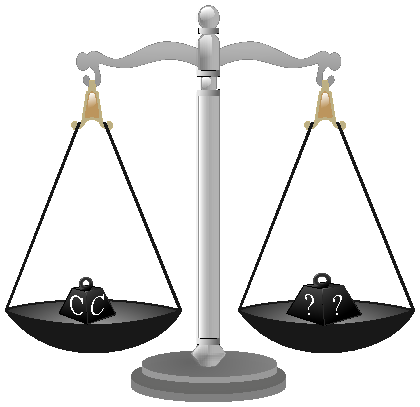
\includegraphics[width=0.2\linewidth]{balancingAct/balanceScale09.pdf}\\J\end{tabular}
    \begin{tabular}{c}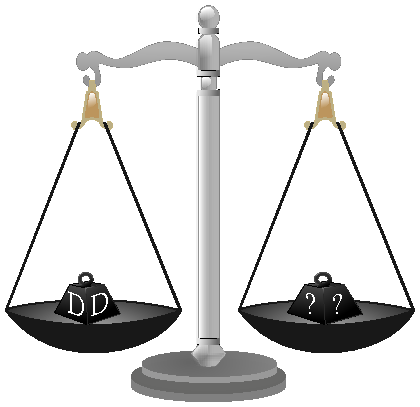
\includegraphics[width=0.2\linewidth]{balancingAct/balanceScale27.pdf}\\L\end{tabular}
  \end{center}
  \begin{center}
    \begin{tabular}{c}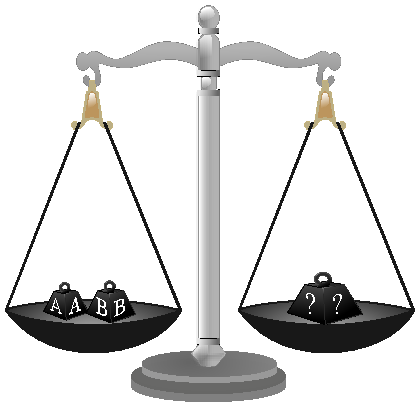
\includegraphics[width=0.2\linewidth]{balancingAct/balanceScale04.pdf}\\M\end{tabular}
    \begin{tabular}{c}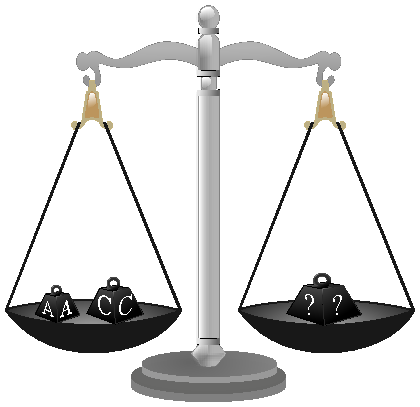
\includegraphics[width=0.2\linewidth]{balancingAct/balanceScale10.pdf}\\O\end{tabular}
    \begin{tabular}{c}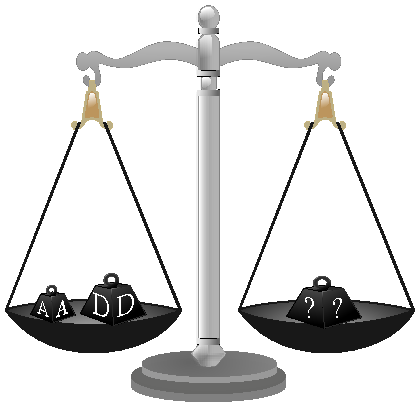
\includegraphics[width=0.2\linewidth]{balancingAct/balanceScale28.pdf}\\E\end{tabular}
    \begin{tabular}{c}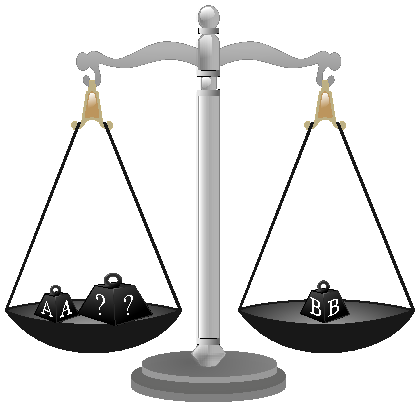
\includegraphics[width=0.2\linewidth]{balancingAct/balanceScale02.pdf}\\O\end{tabular}
  \end{center}
  \begin{center}
    \begin{tabular}{c}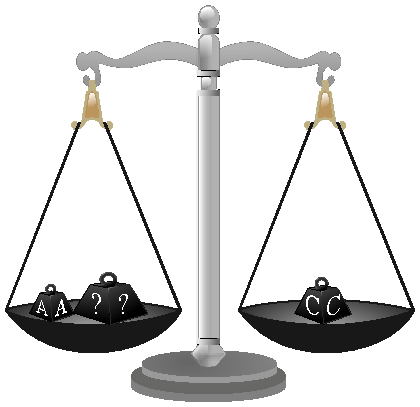
\includegraphics[width=0.2\linewidth]{balancingAct/balanceScale08.pdf}\\N\end{tabular}
    \begin{tabular}{c}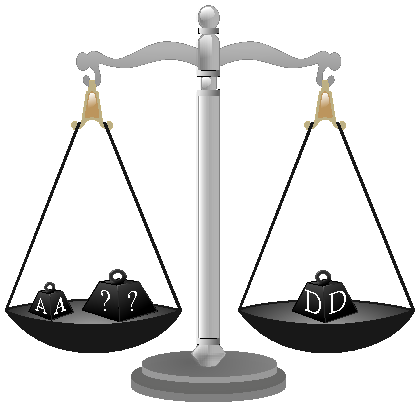
\includegraphics[width=0.2\linewidth]{balancingAct/balanceScale26.pdf}\\O\end{tabular}
    \begin{tabular}{c}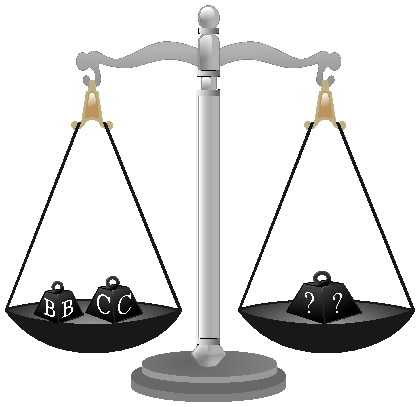
\includegraphics[width=0.2\linewidth]{balancingAct/balanceScale12.pdf}\\W\end{tabular}
    \begin{tabular}{c}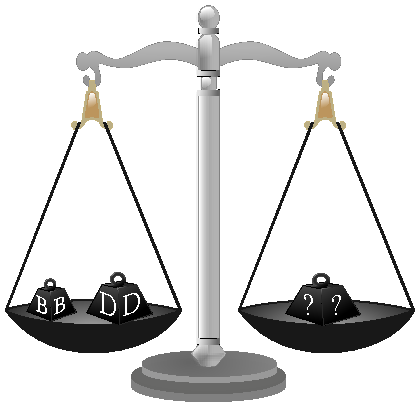
\includegraphics[width=0.2\linewidth]{balancingAct/balanceScale30.pdf}\\C\end{tabular}
  \end{center}
  \begin{center}
    \begin{tabular}{c}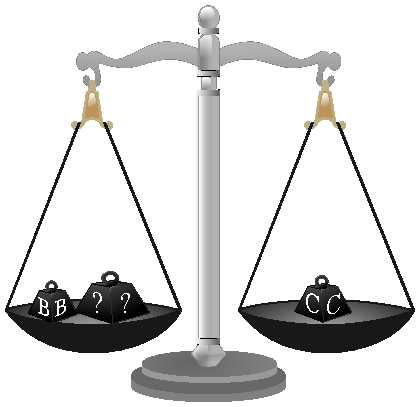
\includegraphics[width=0.2\linewidth]{balancingAct/balanceScale06.pdf}\\Y\end{tabular}
    \begin{tabular}{c}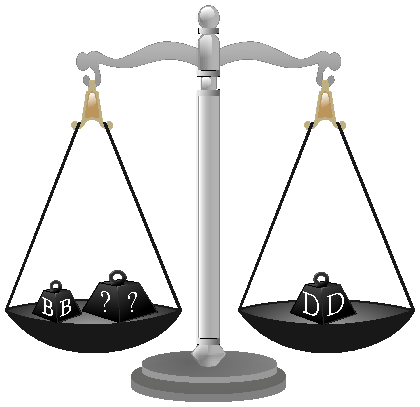
\includegraphics[width=0.2\linewidth]{balancingAct/balanceScale24.pdf}\\T\end{tabular}
    \begin{tabular}{c}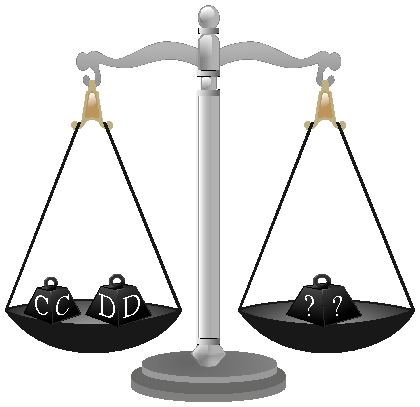
\includegraphics[width=0.2\linewidth]{balancingAct/balanceScale36.pdf}\\D\end{tabular}
    \begin{tabular}{c}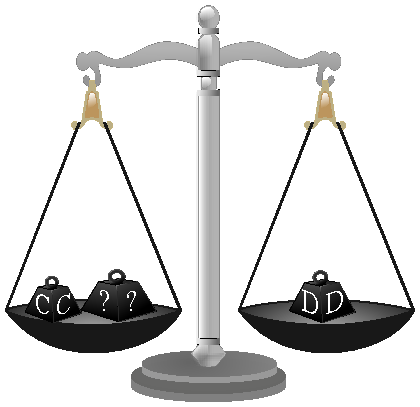
\includegraphics[width=0.2\linewidth]{balancingAct/balanceScale18.pdf}\\G\end{tabular}
  \end{center}
  \begin{center}
    \begin{tabular}{c}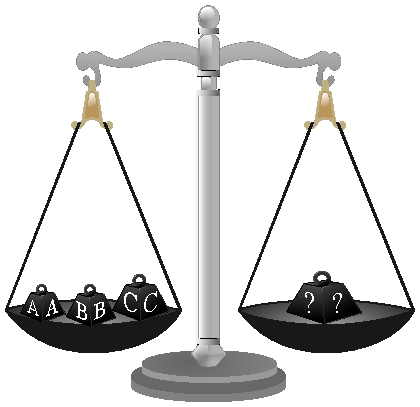
\includegraphics[width=0.2\linewidth]{balancingAct/balanceScale13.pdf}\\O\end{tabular}
    \begin{tabular}{c}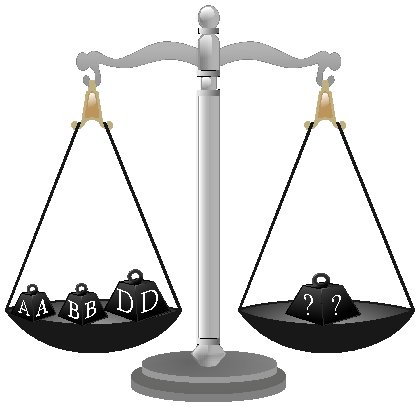
\includegraphics[width=0.2\linewidth]{balancingAct/balanceScale31.pdf}\\D\end{tabular}
    \begin{tabular}{c}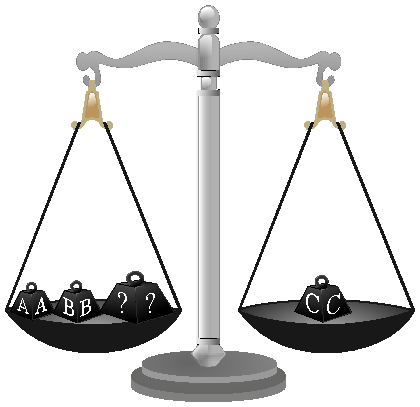
\includegraphics[width=0.2\linewidth]{balancingAct/balanceScale05.pdf}\\A\end{tabular}
    \begin{tabular}{c}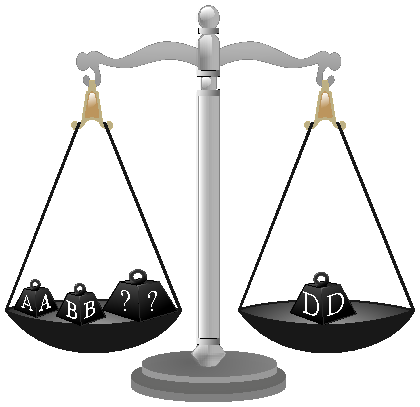
\includegraphics[width=0.2\linewidth]{balancingAct/balanceScale23.pdf}\\I\end{tabular}
  \end{center}
  \begin{center}
    \begin{tabular}{c}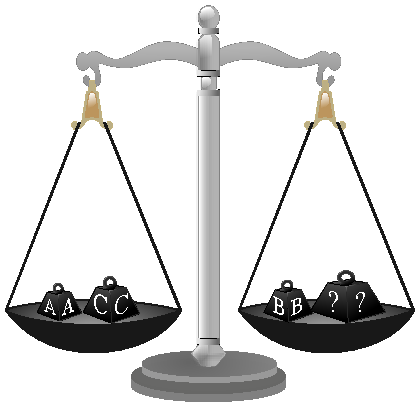
\includegraphics[width=0.2\linewidth]{balancingAct/balanceScale07.pdf}\\E\end{tabular}
    \begin{tabular}{c}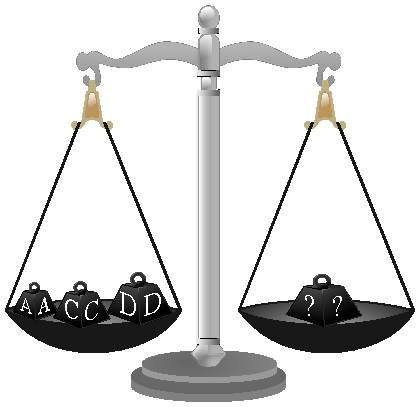
\includegraphics[width=0.2\linewidth]{balancingAct/balanceScale37.pdf}\\H\end{tabular}
    \begin{tabular}{c}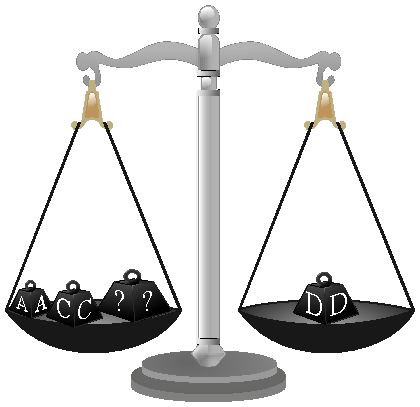
\includegraphics[width=0.2\linewidth]{balancingAct/balanceScale17.pdf}\\N\end{tabular}
    \begin{tabular}{c}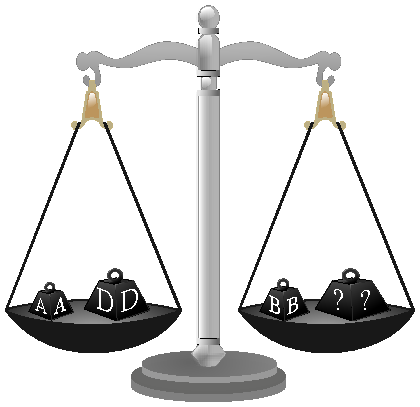
\includegraphics[width=0.2\linewidth]{balancingAct/balanceScale25.pdf}\\H\end{tabular}
  \end{center}
  \begin{center}
    \begin{tabular}{c}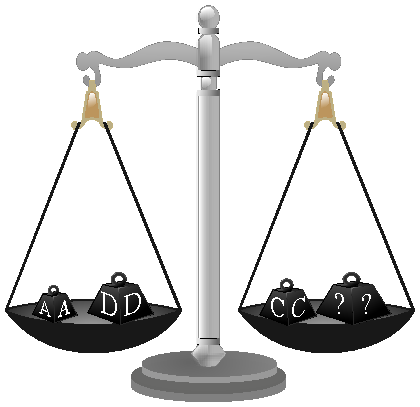
\includegraphics[width=0.2\linewidth]{balancingAct/balanceScale19.pdf}\\O\end{tabular}
    \begin{tabular}{c}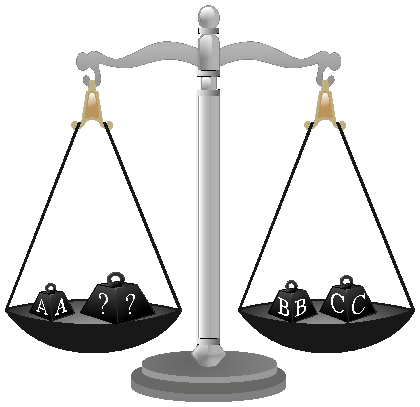
\includegraphics[width=0.2\linewidth]{balancingAct/balanceScale11.pdf}\\Y\end{tabular}
    \begin{tabular}{c}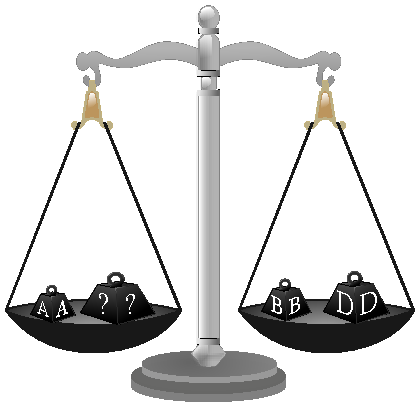
\includegraphics[width=0.2\linewidth]{balancingAct/balanceScale29.pdf}\\M\end{tabular}
    \begin{tabular}{c}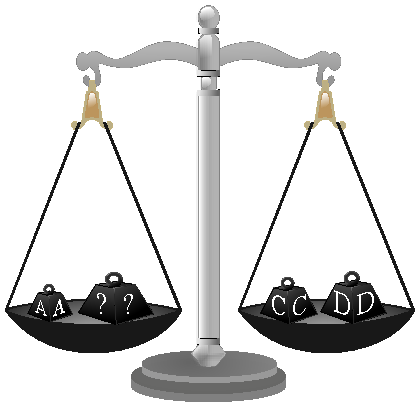
\includegraphics[width=0.2\linewidth]{balancingAct/balanceScale35.pdf}\\L\end{tabular}
  \end{center}
  \begin{center}
    \begin{tabular}{c}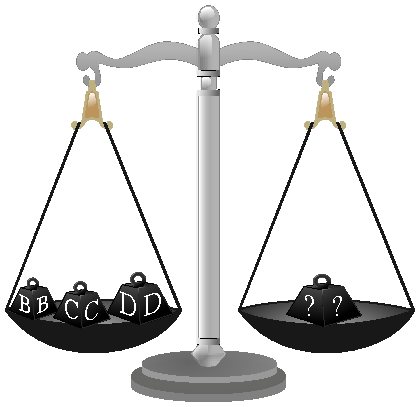
\includegraphics[width=0.2\linewidth]{balancingAct/balanceScale39.pdf}\\R\end{tabular}
    \begin{tabular}{c}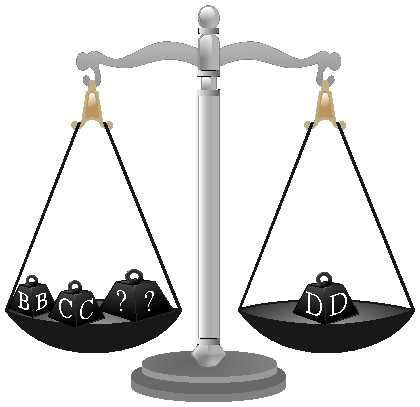
\includegraphics[width=0.2\linewidth]{balancingAct/balanceScale15.pdf}\\K\end{tabular}
    \begin{tabular}{c}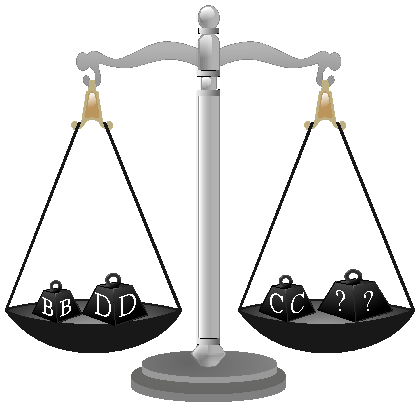
\includegraphics[width=0.2\linewidth]{balancingAct/balanceScale21.pdf}\\T\end{tabular}
    \begin{tabular}{c}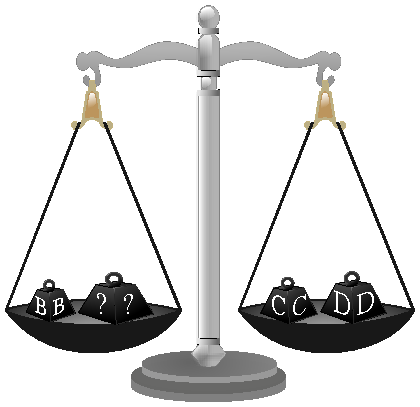
\includegraphics[width=0.2\linewidth]{balancingAct/balanceScale33.pdf}\\N\end{tabular}
  \end{center}
  \begin{center}
    \begin{tabular}{c}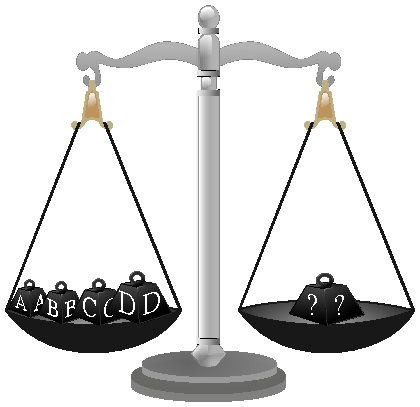
\includegraphics[width=0.2\linewidth]{balancingAct/balanceScale40.pdf}\\E\end{tabular}
    \begin{tabular}{c}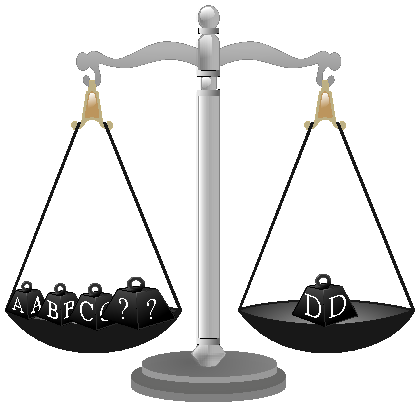
\includegraphics[width=0.2\linewidth]{balancingAct/balanceScale14.pdf}\\R\end{tabular}
    \begin{tabular}{c}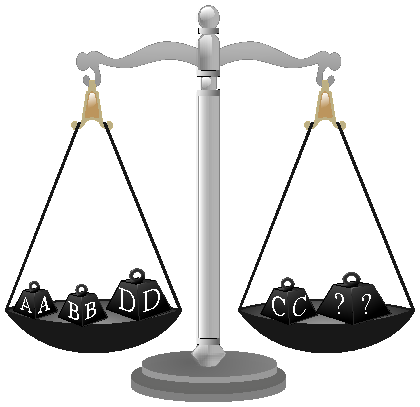
\includegraphics[width=0.2\linewidth]{balancingAct/balanceScale22.pdf}\\W\end{tabular}
    \begin{tabular}{c}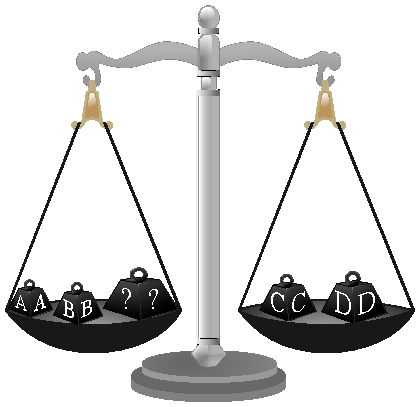
\includegraphics[width=0.2\linewidth]{balancingAct/balanceScale32.pdf}\\O\end{tabular}
  \end{center}
  \begin{center}
    \begin{tabular}{c}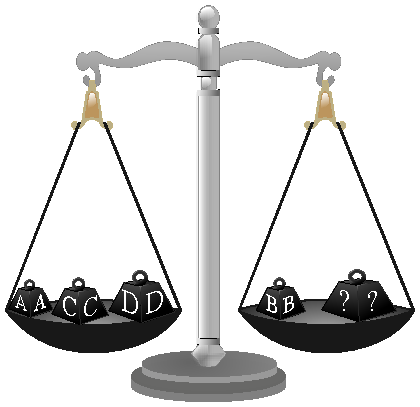
\includegraphics[width=0.2\linewidth]{balancingAct/balanceScale34.pdf}\\A\end{tabular}
    \begin{tabular}{c}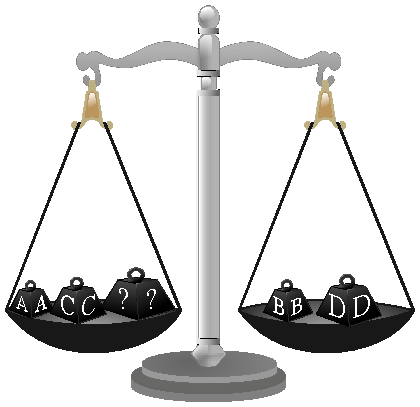
\includegraphics[width=0.2\linewidth]{balancingAct/balanceScale20.pdf}\\U\end{tabular}
    \begin{tabular}{c}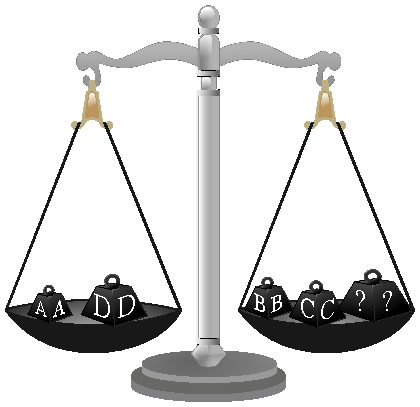
\includegraphics[width=0.2\linewidth]{balancingAct/balanceScale16.pdf}\\I\end{tabular}
    \begin{tabular}{c}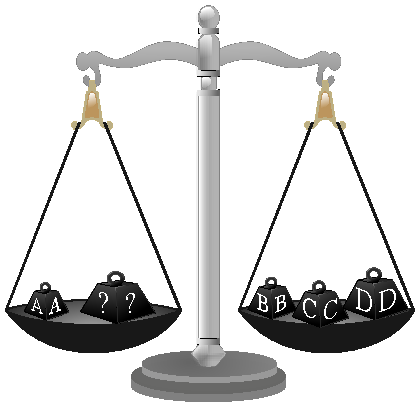
\includegraphics[width=0.2\linewidth]{balancingAct/balanceScale38.pdf}\\E\end{tabular}
  \end{center}

\end{puzzle}

\begin{extraPuzzle}
  We hope you didn't become unbalanced trying to puzzle that one out.

  Here's another balancing challenge. This time you have twelve
  indistinguishable kettlebells, except that one kettlebell has a very
  slightly different weight than the other eleven.
  You don't know if it is heavier or
  lighter. The balance scale can support as many kettlebells on either
  side as you'd like.

  \begin{center}
    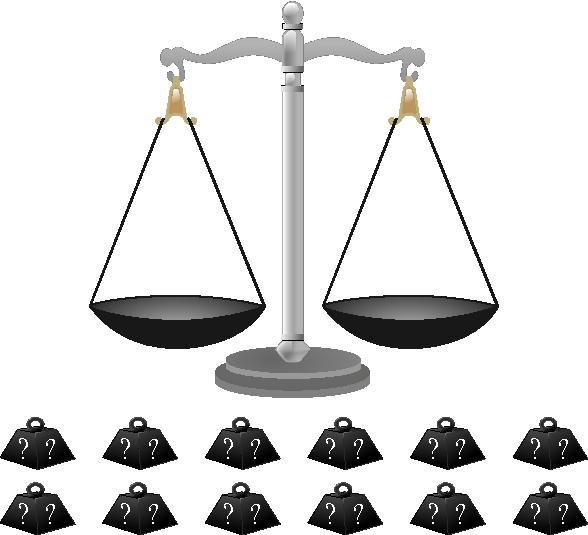
\includegraphics[width=0.7\linewidth]{balancingAct/balanceScaleExtra.pdf}
  \end{center}

  How many times must you use the balance scale to definitively prove
  which kettlebell has the different weight, as well as determine if it
  is heavier or lighter than the other kettlebells?
  Report your best guess to Game HQ, and the team(s) closest to the correct
  answer \textit{without going under} will receive \(50\) points.
\end{extraPuzzle}